\section{Threat Model}
\label{Adversary Model}

We align our threat model with the same basic assumptions as described in~\cite{veen:typearmor}. 
More precisely, we assume a resourceful attacker that has read and write access to the data 
sections of the attacked program binary. We also assume that the protected binary does not contain 
self-modifying code, handcrafted assembly or any kind of obfuscation. We also consider pages 
to be either writable or executable but not both at the same time. Further, we assume 
that the attacker has the ability to execute a memory corruption to hijack the program
control flow. Finally, the analyzed program binary is not hand-crafted and the compiler
which was used to generate the binary adheres to one of the 
standard calling conventions mentioned in \cref{chapter:Introduction}.

\begin{center}
\begin{figure*}[t!]
\centering
   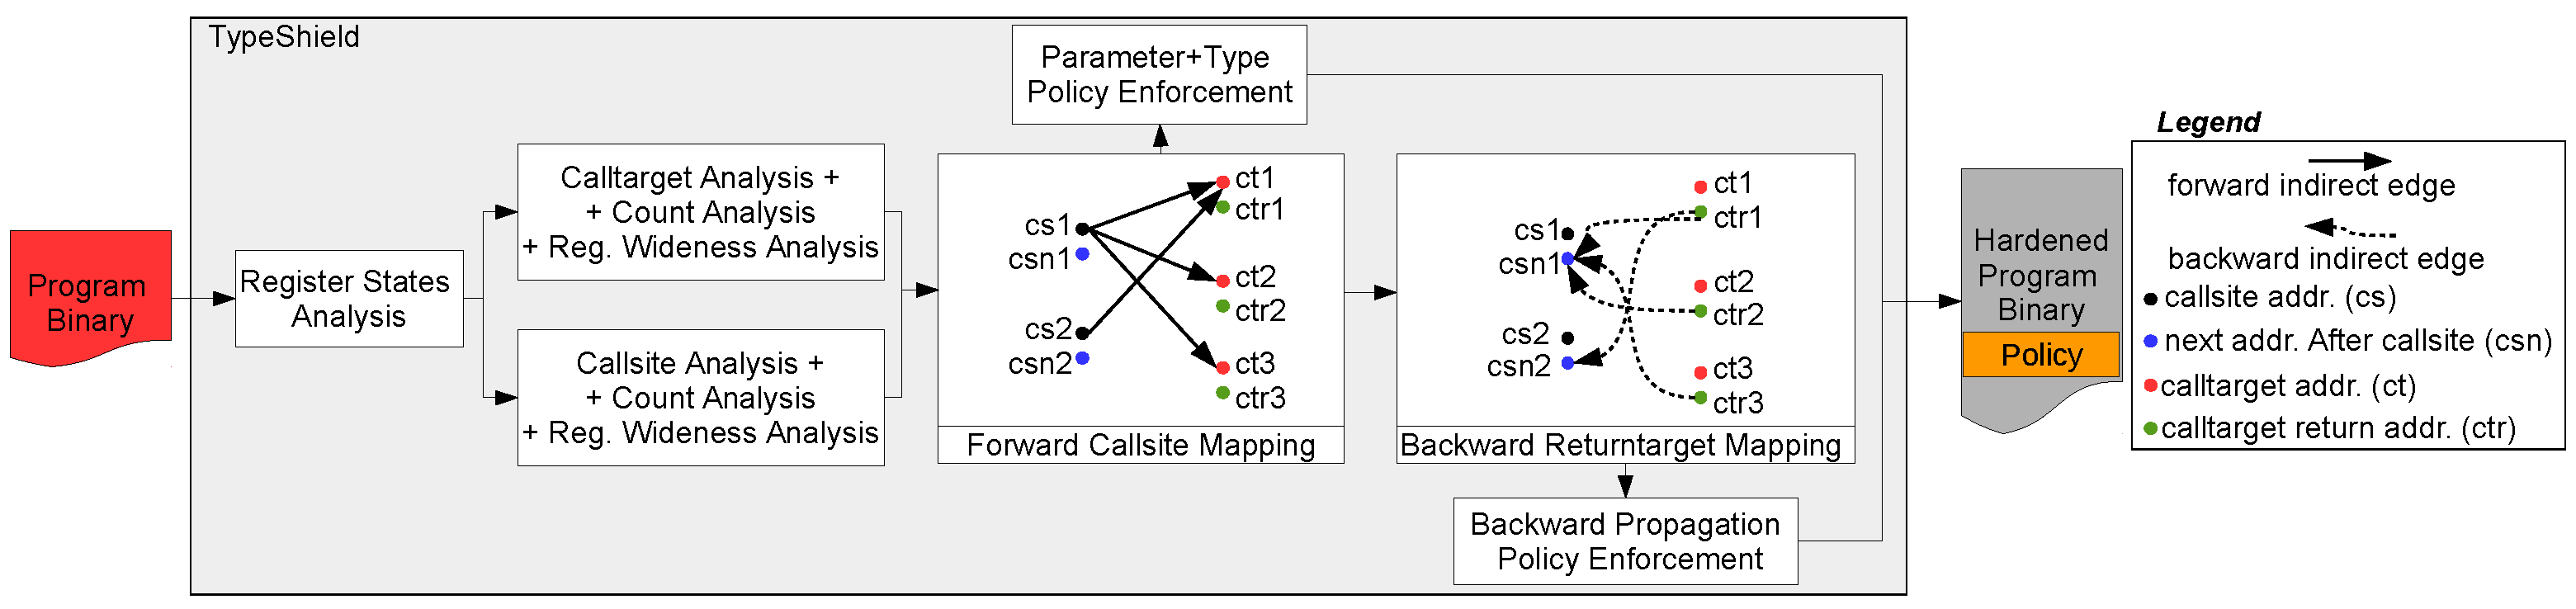
\includegraphics[width=.88\textwidth]{figures/overview.pdf}
    \caption{Overview of the main steps performed by \textsc{TypeShield} when hardening a program binary.}
    \label{System overview.}
    \vspace{-.5cm}
 \end{figure*}
\end{center}